\author[Tommaso Giani]{}
\institute{Nikhef}
\subsection{Positivity}

\begin{frame}{Positivity - Implementation}
	Quarks, anti-quarks and gluon $\overline{MS}$ PDFs $q_k$ have to be positive: we add a term in the $\chi^2$ penalizing negative distributions
	\begin{align*}
		\label{eq:chi2pos_integ}
		\chi^2_{tot} = \chi^2_{exp} + \sum_k\, \chi^2_{k,\text{pos}}\,,
	\end{align*}

	\begin{align*}
		\chi^2_{k,pos} = \Lambda_k \,\sum_i \,\Theta\left(-q_k\left(x_i,Q^2\right)\right)\,,\,\,\,\,\,\,
		\text{with}\,\,\,\,\,\,\,
		\Theta\left(t\right) = 
		\begin{cases}
			t \,\,\,\,\,\,\text{if}\,\,\,\, t>0 \\
			0\,\,\,\,\,\,\,\text{if}\,\,\,\, t<0
		\end{cases}\,.
	\end{align*} 
	\begin{figure}[h!]
		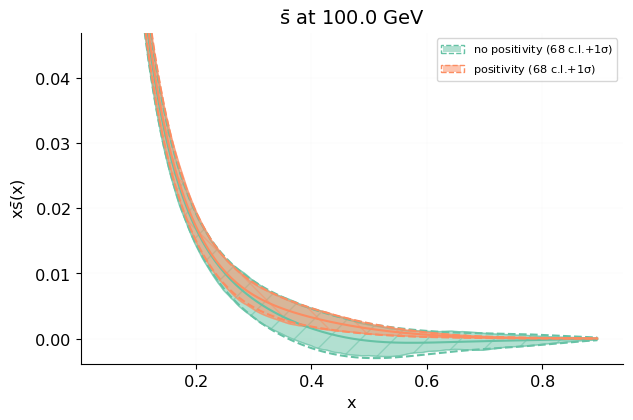
\includegraphics[scale=0.32]{pos_integ/plot_pdfs_bars_pos.png}
		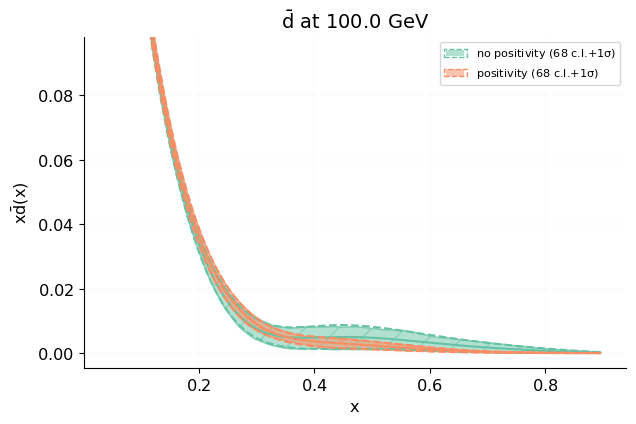
\includegraphics[scale=0.32]{pos_integ/plot_pdfs_bard_pos.png}
	\end{figure}
\end{frame}


\subsection{Integrability}
\begin{frame}{Integrability}
	In order to satisfy valence and Gottfried sum rules the distributions $ q_k =V, V_3, V_8, T_3, T_8$ have to be integrable at small-$x$
	\begin{align*}
		\lim_{x\rightarrow 0} xq_k\left(x,Q_0^2\right) = 0\,.%\,,\,\,\,\,\,\,\,\longrightarrow\,\,\,\,\,\,\, |xq_k|_{x\sim 0} \ll |xq_k|_{x=x_{\text{peak}}}
	\end{align*}
	Similarly to what done for positivity, we add to the total $\chi^2$ a penalty of the form
	\begin{align*}
		\chi^2_{k,integ} = \Lambda_k \,\sum_i \,\left[x_i\,q_k\left(x_i,Q^2\right)\right]^2\,.
	\end{align*}


	\begin{figure}[h!]
		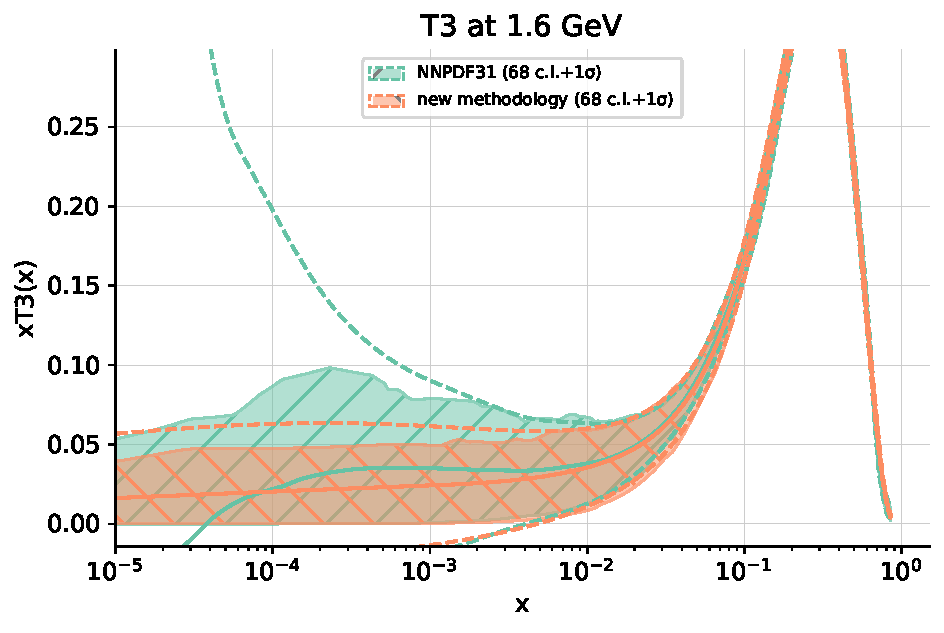
\includegraphics[scale=0.32]{pos_integ/plot_pdfs_T3_integ.pdf}
		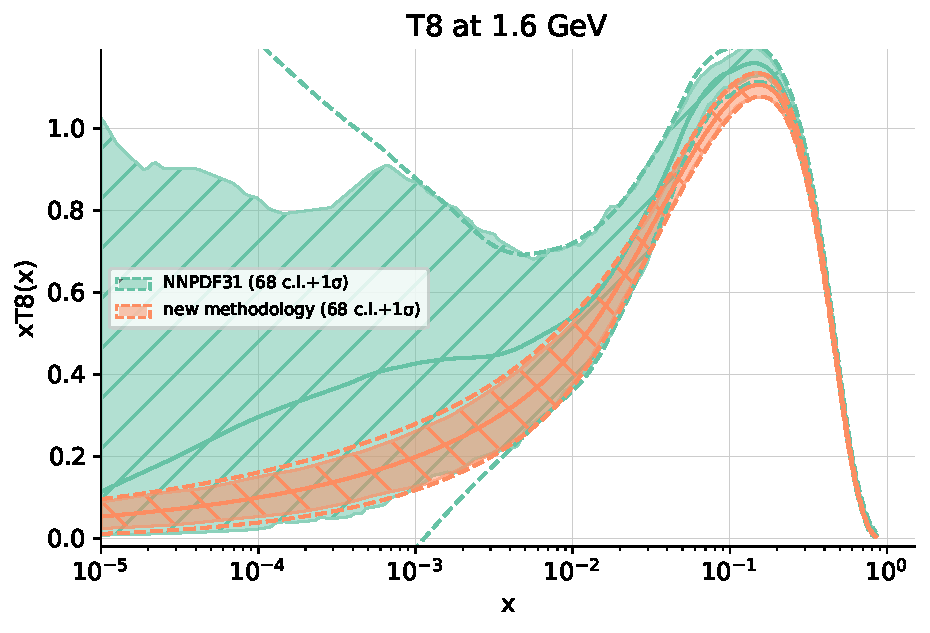
\includegraphics[scale=0.32]{pos_integ/plot_pdfs_T8_integ.pdf}
	\end{figure}

\end{frame}

\subsection{Architecture and fitbasis}
\begin{frame}{Fitbasis}
	\begin{columns}
		\begin{column}{0.55\textwidth}
			\begin{figure}[h!]
				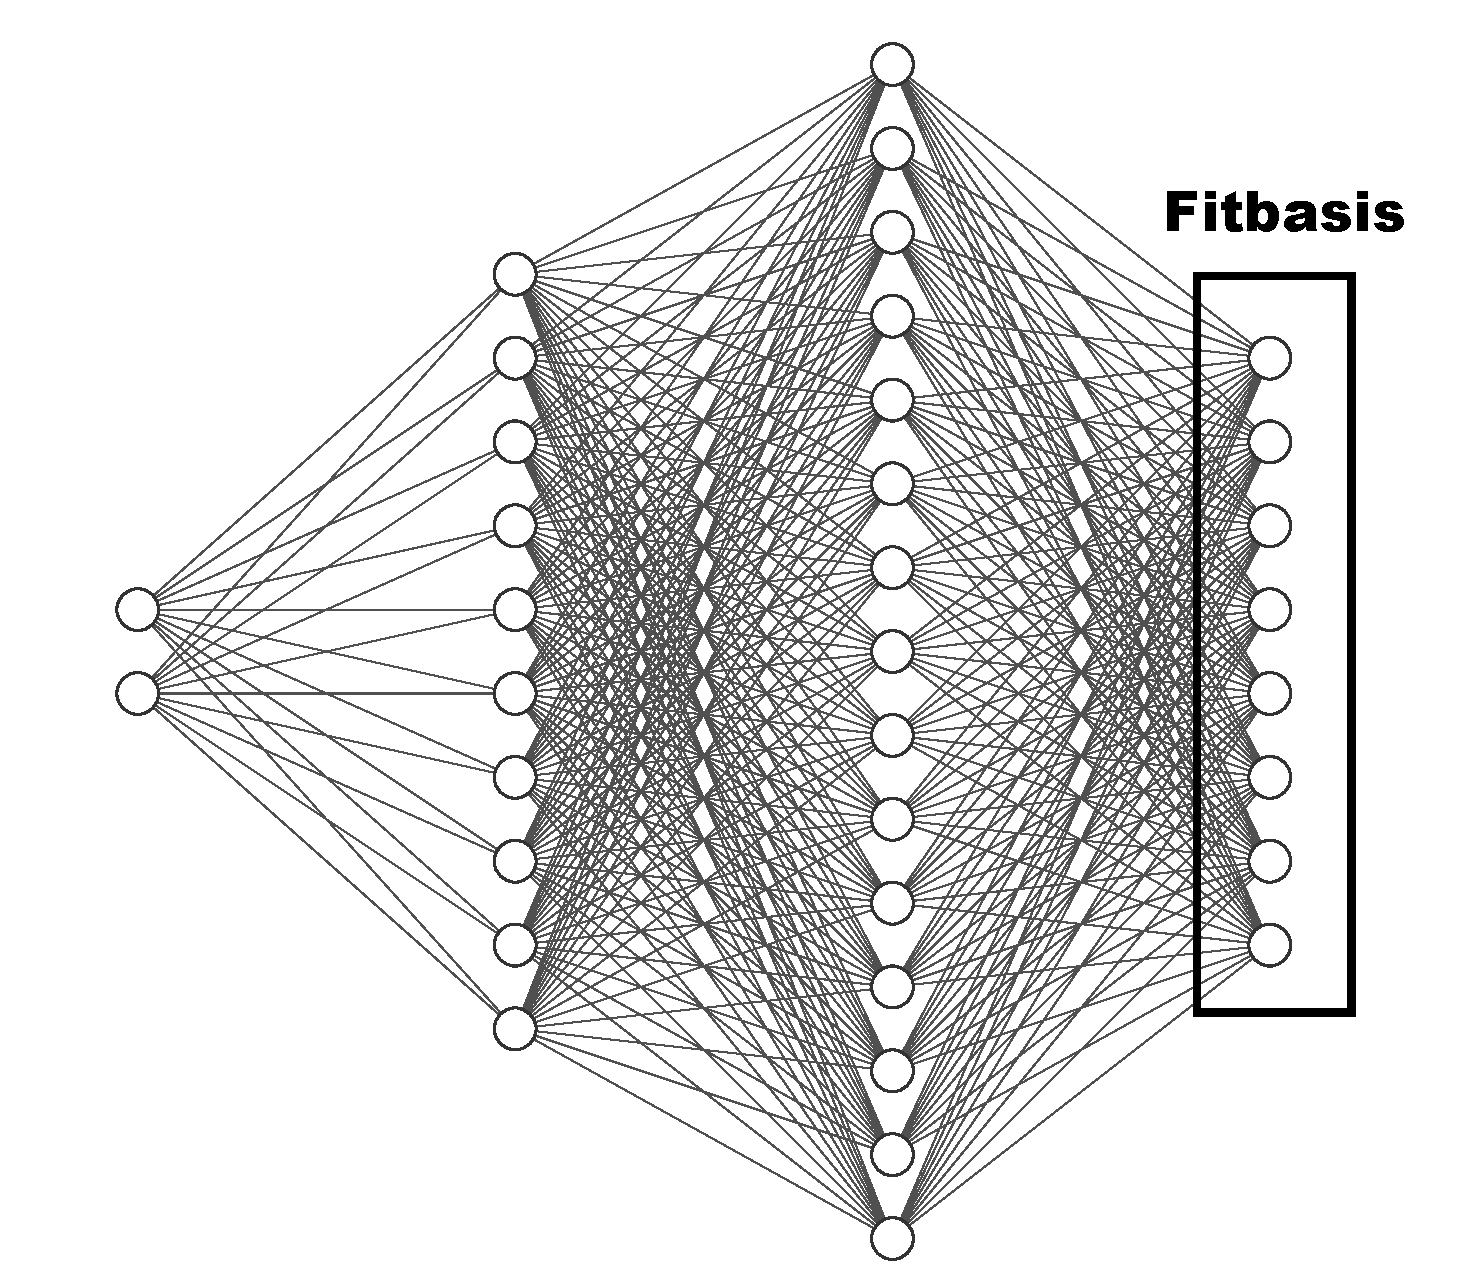
\includegraphics[scale=0.20]{pos_integ/output.pdf}
			\end{figure}
		\end{column}
		\begin{column}{0.45\textwidth}
			% Define block styles
		\tikzstyle{decision} = [diamond, draw, fill=blue!20, 
		text width=4.5em, text badly centered, node distance=3cm, inner sep=0pt]
	\tikzstyle{block} = [rectangle, draw,  
		text width=5em, text centered, rounded corners, minimum height=4em]
	\tikzstyle{line} = [draw, -latex']
	\tikzstyle{cloud} = [draw, ellipse,fill=red!20, node distance=3cm,
		minimum height=2em]
	\centering    
	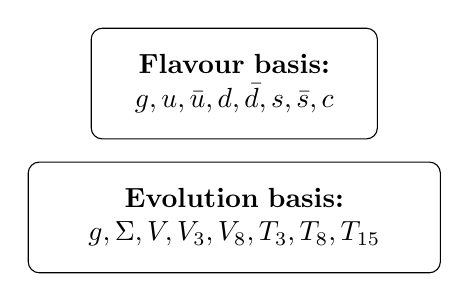
\begin{tikzpicture}[node distance = 1.7cm]
		% Place nodes
		\node [block, text width=3.4cm] (FL) {\textbf{Flavour basis:} \\$g, u, \bar{u}, d, \bar{d}, s, \bar{s}, c$};
		\node [block, text width=5.0cm, below of=FL] (EV) {\textbf{Evolution basis:} \\$g, \Sigma, V, V_3, V_8, T_3, T_8, T_{15}$};
	\end{tikzpicture}
	\end{column}
\end{columns}
\begin{itemize}
	\item NNPDF4.0 will be hyper-optimized in the evolution basis \newline
	\item the final results should not depend on the details of the methodology \\
	$\rightarrow$ fitbasis independence studies \newline
	\item independently on the basis choice the same physical constraints have to be satisfied: positivity and integrability
\end{itemize}
\end{frame}



